%% BioMed_Central_Tex_Template_v1.06
%%                                      %
%  bmc_article.tex            ver: 1.06 %
%                                       %

%%IMPORTANT: do not delete the first line of this template

%%%%%%%%%%%%%%%%%%%%%%%%%%%%%%%%%%%%%%%%%
%%                                     %%
%%  LaTeX template for BioVis 2014  %%
%%      article submissions     %%
%%          adapted from BMC    %%
%%          <8 Jan 2014>              %%
%% Liz Marai (g.elisabeta.marai@gmail.com) %%
%%                                     %%
%%%%%%%%%%%%%%%%%%%%%%%%%%%%%%%%%%%%%%%%%


%%%%%%%%%%%%%%%%%%%%%%%%%%%%%%%%%%%%%%%%%%%%%%%%%%%%%%%%%%%%%%%%%%%%%
%%                                                                 %%
%%%%%%%%%%%%%%%%%%%%%%%%%%%%%%%%%%%%%%%%%%%%%%%%%%%%%%%%%%%%%%%%%%%%%

%%% additional documentclass options:
%  [doublespacing]
%  [linenumbers]   - put the line numbers on margins

%%% loading packages, author definitions

\documentclass[twocolumn]{bmcart}% uncomment this for twocolumn layout 



%%% Load packages
%\usepackage{amsthm,amsmath}
%\RequirePackage{natbib}
%\RequirePackage{hyperref}
\usepackage[utf8]{inputenc} %unicode support
%\usepackage[applemac]{inputenc} %applemac support if unicode package fails
%\usepackage[latin1]{inputenc} %UNIX support if unicode package fails
\usepackage{graphicx}

%%%%%%%%%%%%%%%%%%%%%%%%%%%%%%%%%%%%%%%%%%%%%%%%%
%%                                             %%
%%  If you wish to display your graphics for   %%
%%  your own use using includegraphic or       %%
%%  includegraphics, then comment out the      %%
%%  following two lines of code.               %%
%%%%%%%%%%%%%%%%%%%%%%%%%%%%%%%%%%%%%%%%%%%%%%%%%


%\def\includegraphic{}
%\def\includegraphics{}



%%% Put your definitions there:
\startlocaldefs
\endlocaldefs


%%% Begin ...
\begin{document}

%%% Start of article front matter
\begin{frontmatter}

\begin{fmbox}
\dochead{Research}

%%%%%%%%%%%%%%%%%%%%%%%%%%%%%%%%%%%%%%%%%%%%%%
%%                                          %%
%% Enter the title of your article here     %%
%%                                          %%
%%%%%%%%%%%%%%%%%%%%%%%%%%%%%%%%%%%%%%%%%%%%%%

\title{SketchBio: A Scientist's 3D Interface for Molecular Modeling and Animation}

%%%%%%%%%%%%%%%%%%%%%%%%%%%%%%%%%%%%%%%%%%%%%%
%%                                          %%
%% Do not enter the authors here for        %%
%%  a double-blind review. Otherwise        %%
%% specify information, if available,       %%
%% in the form:                             %%
%%   <key>={<id1>,<id2>}                    %%
%%   <key>=                                 %%
%% Comment or delete the keys which are     %%
%% not used. Repeat \author command as much %%
%% as required.                             %%
%%                                          %%
%%%%%%%%%%%%%%%%%%%%%%%%%%%%%%%%%%%%%%%%%%%%%%
\author[
     addressref={aff1},
  % noteref={n2},
   email={swaldon@cs.unc.edu}
]{\inits{SW}\fnm{Shawn} \snm{Waldon}}
\author[
   addressref={aff1},                   % id's of addresses, e.g. {aff1,aff2}
   %corref={aff1},                       % id of corresponding address, if any
   %noteref={n1},                        % id's of article notes, if any
  email={taylorr@cs.unc.edu}   % email address
]{\inits{RT}\fnm{Russell} \snm{Taylor} \suffix{II}}
\author[
	addressref={aff1},
	email={pthomps@live.unc.edu}
]{\inits{PT}\fnm{Peter} \snm{Thompson}}

%%%%%%%%%%%%%%%%%%%%%%%%%%%%%%%%%%%%%%%%%%%%%%
%%                                          %%
%% Enter the authors' addresses here        %%
%%                                          %%
%% Repeat \address commands as much as      %%
%% required.                                %%
%%                                          %%
%%%%%%%%%%%%%%%%%%%%%%%%%%%%%%%%%%%%%%%%%%%%%%

\address[id=aff1]{%                           % unique id
  \orgname{University of North Carolina at Chapel Hill}, % university, etc
  \postcode{27599}                                % post or zip code
  \city{Chapel Hill, NC},                              % city
  \cny{US}                                    % country
}
%\address[id=aff2]{%                           % unique id
%  \orgname{Anonymous Also}, % university, etc
%  \street{210 South Bouquet},                     %
%  \postcode{15260}                                % post or zip code
%  \city{Williamsburg},                              % city
%  \cny{UK}                                    % country
%}


%%%%%%%%%%%%%%%%%%%%%%%%%%%%%%%%%%%%%%%%%%%%%%
%%                                          %%
%% Enter short notes here                   %%
%%                                          %%
%% Short notes will be after addresses      %%
%% on first page.                           %%
%%                                          %%
%%%%%%%%%%%%%%%%%%%%%%%%%%%%%%%%%%%%%%%%%%%%%%

\begin{artnotes}
%\note{Sample of title note}     % note to the article
%\note[id=n1]{Equal contributor} % note, connected to author
%\note[id=n2]{Equal contributor} % note, connected to author
%\note[id=n3]{Equal contributor} % note, connected to author
%\note[id=n4]{Project leader and equal contributor} % note, connected to author
\end{artnotes}

\end{fmbox}% comment this for two column layout

%%%%%%%%%%%%%%%%%%%%%%%%%%%%%%%%%%%%%%%%%%%%%%
%%                                          %%
%% The Abstract begins here                 %%
%%                                          %%
%% Please refer to the Instructions for     %%
%% authors on http://www.biomedcentral.com  %%
%% and include the section headings         %%
%% accordingly for your article type.       %%
%%                                          %%
%%%%%%%%%%%%%%%%%%%%%%%%%%%%%%%%%%%%%%%%%%%%%%

\begin{abstractbox}

\begin{abstract} % abstract, must be under 350 words
%\parttitle{First part title} %if any
%Text for this section.

\parttitle{Background} Because of the difficulties involved in learning and using 3D modeling and rendering software, many scientists hire professional computer programmers and/or animators to work with them to create models and animations rather than use these programs themselves.  This indirection both slows the discovery process and provides opportunities for miscommunication. As toolsmiths, our aim is to provide scientists with a tool that is so rapid to learn and powerful to use that they can create these models and animations themselves. 

\parttitle{Results}  SketchBio includes novel interaction and computational techniques that directly support the construction of macromolecular structures: crystal by example and pose-mode physics both provide improved modeling capabilities and both enable more-rapid collision detection.  Spring connectors show unspecified interactions and support semi-automatic structure formation.

\parttitle{Conclusions} SketchBio is a new tool that enables scientists to rapidly construct and validate hypothetical macromolecular structures, to animate these structures, and to produce high-quality rendered animations.  It has been tested and shown to meet its design goals: (1) Scientists can construct models and animations on their own. (2) Structures and animations can be rapidly constructed, modified, and tested. (3) State-of-the-art tools and methods are harnessed rather than reimplemented.

%\parttitle{Second part title} %if any
%Text for this section.
\end{abstract}

%%%%%%%%%%%%%%%%%%%%%%%%%%%%%%%%%%%%%%%%%%%%%%
%%                                          %%
%% The keywords begin here                  %%
%%                                          %%
%% Put each keyword in separate \kwd{}.     %%
%%                                          %%
%%%%%%%%%%%%%%%%%%%%%%%%%%%%%%%%%%%%%%%%%%%%%%

\begin{keyword}
\kwd{Molecular Modelling}
\kwd{Animation}
\kwd{Collision Detection}
\end{keyword}

% MSC classifications codes, if any
%\begin{keyword}[class=AMS]
%\kwd[Primary ]{}
%\kwd{}
%\kwd[; secondary ]{}
%\end{keyword}

\end{abstractbox}
%
%\end{fmbox}% uncomment this for twcolumn layout

\end{frontmatter}

%%%%%%%%%%%%%%%%%%%%%%%%%%%%%%%%%%%%%%%%%%%%%%
%%                                          %%
%% The Main Body begins here                %%
%%                                          %%
%% Please refer to the instructions for     %%
%% authors on:                              %%
%% http://www.biomedcentral.com/info/authors%%
%% and include the section headings         %%
%% accordingly for your article type.       %%
%%                                          %%
%% See the Results and Discussion section   %%
%% for details on how to create sub-sections%%
%%                                          %%
%% use \cite{...} to cite references        %%
%%  \cite{koon} and                         %%
%%  \cite{oreg,khar,zvai,xjon,schn,pond}    %%
%%  \nocite{smith,marg,hunn,advi,koha,mouse}%%
%%                                          %%
%%%%%%%%%%%%%%%%%%%%%%%%%%%%%%%%%%%%%%%%%%%%%%

%%%%%%%%%%%%%%%%%%%%%%%%% start of article main body
% <put your article body there>


%%%%%%%%%%%%%%%%
%% Background %%
%%
\section*{Background}

In his introduction to the ``Cellular and Molecular Data" session at BioVis 2013, Tom Ferrin identified two open challenges for biology software.  The first was to ``Provide easy-to-use learning tools that can still convey complex structures" and the second was to ``Develop easy-to-use interfaces that permit facile control of models".  We’re developing SketchBio to help scientists think about 3D molecular structures and interactions, to communicate them to others, and to drive microscope simulations for experiment planning and analysis.

We found ourselves repeatedly using 2D hand-drawings of complex 3D structures and their interactions in discussions with our close collaborators in cell biology, pathology, and chemistry, despite the fact that the 3D crystal structures of the proteins making up these structures were known.  Hanging David Goodsell's excellent ``Molecular Machinery" poster \cite{Goodsell} showing renderings of many of these molecules and their interactions helped to grow our shared understanding of the structures in the mitotic spindle, but real progress was made when we hired an artist to draw 3D scale models of the structures each week and then develop 3D computer models \cite{taylor2012}.

Our group is not alone.  Discussions among collaborators are often done using 2D whiteboard sketches.  Presentations often consist of pasted images and 2D Powerpoint animations.

Because of the difficulties involved in learning and using 3D modeling and rendering software, many scientists hire professional computer programmers and/or animators to work with them to create models and animations rather than use these programs themselves.  This indirection both slows the discovery process and provides opportunities for miscommunication. As toolsmiths, our aim is to provide scientists with a tool that is so rapid to learn and powerful to use that they can create these models and animations themselves.

This paper describes that tool, SketchBio.

\subsection*{Driving Problems}
Fred Brooks points out that the best way to construct a tool that is generally usable is to focus on several very different specific problems and build a tool that solves them.  We are following this approach.

The first driving problem for this project is collaborator Susan Lord's desire to construct a protofibril model based on geometric constraints among a set of fibrinogen monomers.  Based on the crystallized structures of fibrin monomers from different species and on only two sets of known interactions \cite{lord2007fibrinogen}, she sought to construct 3D protofibril structures matching those seen in TEM studies.  Over several months, she and her students worked with Resource staff scientist Joe Hsiao to use the powerful UCSF Chimera tool to construct such a model \cite{lordSubmitted}.  Building this model required repeated iteration of hand-placement of two molecules (using multiple 2D mouse interactions), followed by using replication tools to develop candidate models, which were then evaluated against the data.  Lord's desired use of SketchBio was to construct this protofibril rapidly and semi-automatically by specifying which location on each fibrin should be in close contact with other molecules and by specifying that the molecules do not overlap.  This same capability will enable generation of other self-symmetric structures such as actin filaments and microtubules.

Our second driving problem is comes from Peter Thompson in Sharon Campbell's lab.  Peter wants to construct 3D models and animations of the interaction between actin filaments and vinculin.  He has used SketchBio to reproduce 3D geometry from example structures found in the literature and to generate animated videos to show his hypothetical interactions to colleagues.  He is particularly interested in using SketchBio as a thinking tool to determine how mutations in the vinculin can turn the normally-straight actin filaments into helices.  The resulting optimization algorithms will enable other scientists to semi-automatically construct multi-protein structures that match TEM images.

The third driving problem comes from our collaboration with Kerry Bloom, described above.  As in the Lord case, each step of model generation has required support from an artist, animator, and/or programmer to convert Bloom's concepts and those of his students into geometry for rendering and simulation.  Our program-generated models exhibit more symmetry than the experimental results only because of the difficulty in specifying more complex models that meet the geometric constraints (cohesin loops surrounding four chromatin, no self-intersection or entanglement, etc.).  Bloom needs SketchBio to support (i) the rapid generation of long coarse-grained interacting polymer chains and their connection to coarse-grained models of symmetric microtubules, (ii) the construction of linked but non-colliding protein-chromosome structures, and (iii) production of simulated fluorescence images from the resulting structures.

Our final driving problem also comes from this collaboration.  Many proteins beyond cohesin and condensin contribute to mitosis, and Kerry Bloom is interested in them all.  His lab is able to fluorescently label both these proteins and chromosome locations, and use multi-color or FRET techniques to determine relative distances and orientations between pairs of proteins.  With accurate localization and tracking for 3D images, these techniques provide partial information on the 3D layout of proteins and chromosomes in wild-type and mutant mitotic spindles.  Building matching models requires the development of mass-spring-driven semi-automatic layout of proteins.  This will provide a partial set of constraints for the scientist to construct protein-protein and protein-chromosome complexes that match experimental data.  With these enhancements, SketchBio will be widely useful to other researchers for the generation of hypothetical protein-complex structures from partial data.

We aim to produce a general tool that is widely useful.  Many researchers studying cell structure and physiology seek to construct
and evaluate dynamic models that incorporate random thermal motion as
well as conformational changes induced through intermolecular interactions.
Discovering, testing, and communicating hypotheses about these
interactions requires the development of complex animated 3D structures. Modeling, simulation, and rendering
of these hypothetical scenarios involves using a number of tools and databases (PDB, Pymol, Blender, NAMD, etc.)
and then converting files to pass geometry and animations between tools. It also involves
manual placement and orientation of 3D objects, which is currently done using clunky 2D input devices and by-hand
detection and avoidance of collisions. As a result, it often takes a team months to produce an acceptable
model or animation. We aim to reduce this to a single person working for hours or days.

\subsection*{Prior Work}
\paragraph*{Molecular modeling:}
There are many excellent molecular modeling applications that have been extended to include some aspects of high-quality rendering and animation.  UCSF Chimera \cite{pettersen2004ucsf}, Pymol \cite{pymol2013}, and Visual Molecular Dynamics (VMD) \cite{humphrey1996} are three of the most relevant.  VMD already includes direct force-feedback-based placement and manipulation of molecules.  We considered the approach of extending the interaction and rendering capabilities of one of these tools, but this would mean replicating existing rendering pipelines and techniques that are already implemented elsewhere.  It would also require continual updating as new rendering advances are made.  We instead decided to harness the power of the existing tools through their built-in scripting languages (SketchBio has used both Pymol and Chimera to load, surface, select, and label molecules by partial charge and other inputs).

\paragraph*{Rendering:}
There are also excellent general-purpose rendering programs (such as the commercial Maya and open-source Blender applications) and microscope-simulation rendering tools (such as UNC's Microscope Simulator \cite{quammen2008}).  Several groups are building molecule-specific loaders that plug into these programs, such as Autofill/Autopack/Autocell \cite{Johnson2013}, Molecular Flipbook \cite{flipbook2013}, and Molecular Maya \cite{molecularmaya}.  We also considered this approach, but providing full capability would require replicating the many existing capabilities in molecular modeling tools and tracking new features as they are developed.  We decided to harness the animation and rendering capabilities of Blender using its built-in Python scripting interface.

\paragraph*{Interactive Animation:}
The Molecular Control Toolkit \cite{sabirmolecular} is also aimed at molecular modeling, providing gesture- and speech-based user interface primitives to control motions of molecules with a Kinect or Leap Motion device \cite{sabirmolecular}; they provide an API that can be used to connect their controls to existing molecular modeling applications.  SketchBio uses similar two-handed 6-degree-of-freedom input devices (the Razer Hydra or two WiiMote controllers), adding collision detection and several custom capabilities, and tying the resulting system into existing powerful molecular modeling and rendering tools to produce a complete system for modeling, thinking, and rendering.  Another tool aimed at simplifying the creation of molecular animations, PresentaBALL\cite{nickelspresentaball}, uses an interactive web interface to an existing molecular modeling tool \cite{nickelspresentaball}.  This allows widespread use by non-experts to develop presentation materials for training.  SketchBio provides a custom interface for experts to use as a thinking aid that is tied to a powerful rendering engine to produce animations.

\paragraph*{Interactive Rendering:}
A common bottleneck in interactive modeling and animation applications is the speed of rendering a complex scene.  A key technique in improving the rendering speed of an application is reducing the complexity of the objects that are drawn.  This is done by replacing objects with imposters which are simpler pieces of geometry that result in the same or a very similar result being rendered.  Imposters can be difficult to notice, especially if they are far from the camera and the resulting screen area is small.  One type of imposter is a simplified version of the geometry that is textured to look like the more complex version \cite{decoret2003billboard}\cite{erikson1998simplification}\cite{cohen1998appearance}.  Another common imposter is a square that has a pre-rendered image of the more complex object as its texture.  As long as the viewpoint stays near the same position the discrepancies between this and the actual geometry will be small \cite{aliaga1996visualization}\cite{maciel1995visual}.  The level of simplification of an object can also be dynamically determined according to the amount of the allotted rendering time that is needed to draw each level of detai.  SketchBio uses Chimera and Blender to simplify geometry and the Visualization ToolKit (VTK) library to adjust rendered level of detail \cite{VTKbook}.

\paragraph*{Collision Detection:}
In order to create a model or animation that is useful, collisions between molecules must be detected and handled or reported to the user.  If there are $n$ molecules in the scene, then each of the $n\choose 2$ pairs of molecules must be tested for collisions.  Between each pair of molecules tested, each single unit in one must be tested against each single unit in the other.  This means that collision detection has a complexity of $\mathcal{O}(n^2)$ in the number of primitives since there can be $\mathcal{O}(n^2)$ collisions.  However, there are typically far fewer collisions than potential collisions and so optimizations can reduce the expected complexity.  The best expected complexity uses sweep and prune methods and assumes the primitives are sorted in some dimension to get a complexity of $\mathcal{O}(n + c)$ where c is the number of colliding pairs \cite{tracy2009efficient}.  Described in Tracy, Buss \& Woods is a complex method of keeping the list of primitives sorted in some dimension to avoid the $\mathcal{O}(n lg(n))$ cost of sorting the list at each timestep as objects move \cite{tracy2009efficient}.

A somewhat simpler approach is to use a space partitioning method to rule out tests that do not need to be performed.  Space partitioning can be done using a tree of primitives and the volumes that bound them, called a bounding volume hierarchy.  This approach is used by libraries such as the PQP library created by the UNC GAMMA group \cite{PQP}.  An alternate kind of space partitioning is to divide space into “bins” and group the objects by which bin they are in.  Then only the other primitives in the same bin or very nearby bins need to be tested against them.  This type of algorithm is especially effective on GPUs where many local groups may be run in parallel \cite{oat2008efficient}.

SketchBio directly links to PQP and uses it for basic collision detection.  It extends these techniques in ways that are specific to the kinds of molecular models being formed to gain an additional order of magnitude reduction in collision tests for some objects.

\paragraph*{Mash-ups:}
Individual capabilities of web-based applications such as Google maps and real-estate listing databasese have been effectively combined to provide combination tools that include the best parts of each.  A system for seamless integration of applications for visualization was done by Rungta et. al by adding a layer above all of the applications of interest to pass events back and forth \cite{rungta2013manyvis}.  SketchBio takes a similar approach, using a novel core component that provides interactivity and custom features but using scripting interfaces to harness the significant modeling and rendering capabilities of existing tools into a seamless workflow.

\section*{Methods}

SketchBio is a system for understanding subcellular biology through the building of complex 3D macromolecular structures, and animating the structures over time.

The modeling and rendering of these hypothetical structures currently involves using a number of tools and databases and converting files and data to pass between tools.

SketchBio consolidates state-of-the-art tools and libraries into a seamless workflow, enabling two-handed 6-degree-of-freedom real-time direct interaction with groups of molecules.  It adds several novel features that accelerate this workflow for three different user groups.

\subsection*{System Overview}

Figure \ref{fig:actin_vinculin} shows a screenshot of the SketchBio user interface with a group of three actin molecules (left) and the tail region of a vinculin molecule (right).  The small white spheres in the center represent the two tracked hand-held controllers. Status information about the current system state is shown in the lower left.  Animation timepoint in seconds is shown in the lower right.

\begin{figure}[ht]
\centering
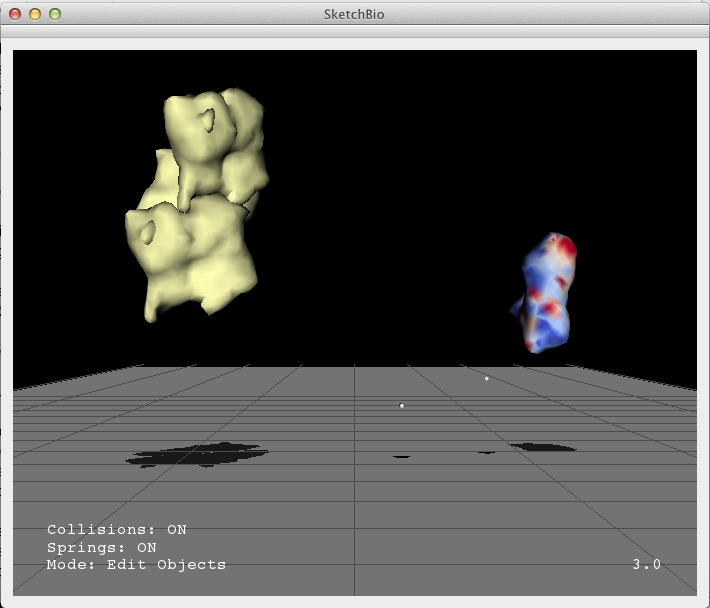
\includegraphics[width=0.9\columnwidth]{actinVinculin.png}
\caption{A screen shot from SketchBio showing three actin monomers on the left colored yellow and the tail region of the vinculin protein on the right colored by surface charge.}
\label{fig:actin_vinculin}
\end{figure}

\subsection*{State-of-the-art Capabilities}

\paragraph*{Bimanual Interaction:}
Bill Buxton and others have described the benefits of two-handed (bimanual) interaction.  He and others observed in \ref{leganchuk1998} that bimanual manipulation brings ``two types of advantages to human-computer interaction: manual and cognitive. Manual benefits come from increased time-motion efficiency, due to the twice as many degrees of freedom simultaneously available to the user. Cognitive benefits arise as a result of reducing the load of mentally composing and visualizing the task at an unnaturally low level imposed by traditional unimanual techniques."

As seen in Figure \ref{fig:two_hands}, SketchBio brings these important benefits to the construction of macromolecular structures.  The entire interface is built around a set of world and root-object manipulation controls in the non-dominant hand and a set of individual-element manipulation controls using the dominant hand.

\begin{figure}[ht]
\centering
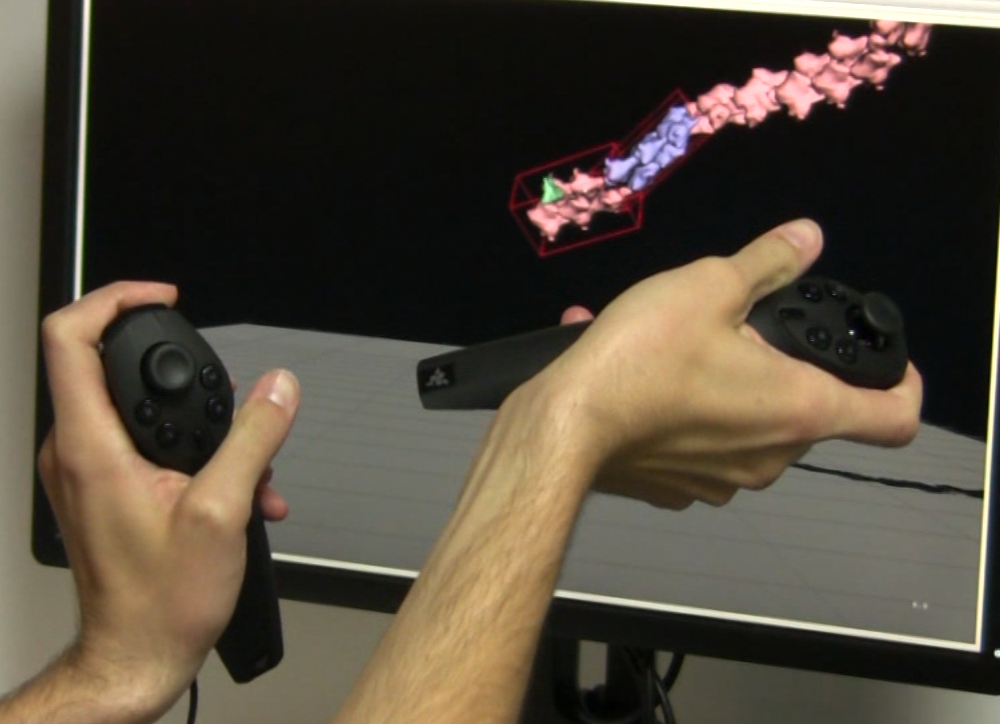
\includegraphics[width=0.9\columnwidth]{two_hands.png}
\caption{The left hand sets the base molecule while the right hand positions the copies in this two-handed construction of an actin fiber.}
\label{fig:two_hands}
\end{figure}

SketchBio uses a pair of Razer Hydra controllers to provide two 6-DOF trackers, each of which also has several buttons, a hi-hat controller, and an analog input.  This enables a very expressive set of verbs (buttons), nouns (selection via 3-DOF positioning), and adjectives (magnitude via analog inputs, viewpoint via hi-hat, and pose via a combined 12-DOF tracking).  This avoids the need for the system to recognize a large set of ambiguous gestures, as is the case for video-based user input.

Using one of the buttons to switch between modes provides a sufficiently-large space of commands that almost all operations can be performed without putting down the controllers.  The keyboard and mouse are used to name proteins and files on initial loading, and to set precise values as needed for one or two operations.

\begin{figure}[h]
\centering
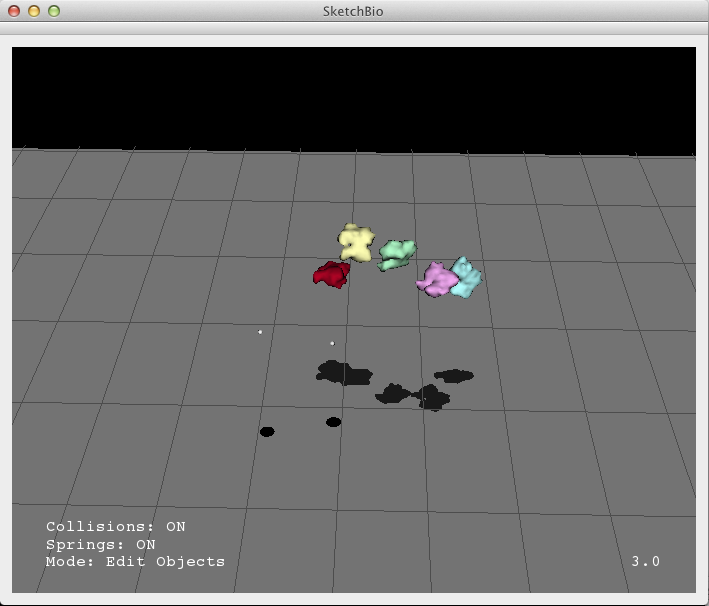
\includegraphics[width=0.9\columnwidth]{shadow_plane.png}
\caption{A screenshot from SketchBio showing colored molecules and a different camera angle to emphasize the shadow plane's effect.}
\label{fig:shadow_plane}
\end{figure}

\paragraph*{Shadows:}
Selection in SketchBio involves moving the tracker to a location within the bounding box of the object, so determining the relative depth between the tracker and the object is an important and often-performed task.  Initial testing of the application revealed that determining the relative depth between an object and the user's hand or between two objects was the most difficult part of using SketchBio.  Because widespread adoption would be limited by requiring stereo displays and head tracking, we sought another solution.   Hendrix and Barfield found the most effective techniques for aiding in depth estimation are a textured plane and lines dropped from the center of an object to the textured plane \cite{Hendrix1995103}.  To provide additional depth cues, SketchBio displays a ground plane that is always rendered below the viewpoint no matter the direction or position of the viewpoint and projects the shadows of objects onto this plane.  The trackers also cast shadows onto this plane (which are darker to highlight them).  SketchBio assumes a light infinitely far away in the default camera's up direction which gives the same absolute position against the textured surface as the drop-lines while also giving information about how close the boundaries of two objects are to each other.  The user can also rotate the camera while leaving the light and shadow plane fixed to get a better understanding of the scene through motion parallax [See Figure \ref{fig:shadow_plane}].

\begin{figure}[h]
\centering
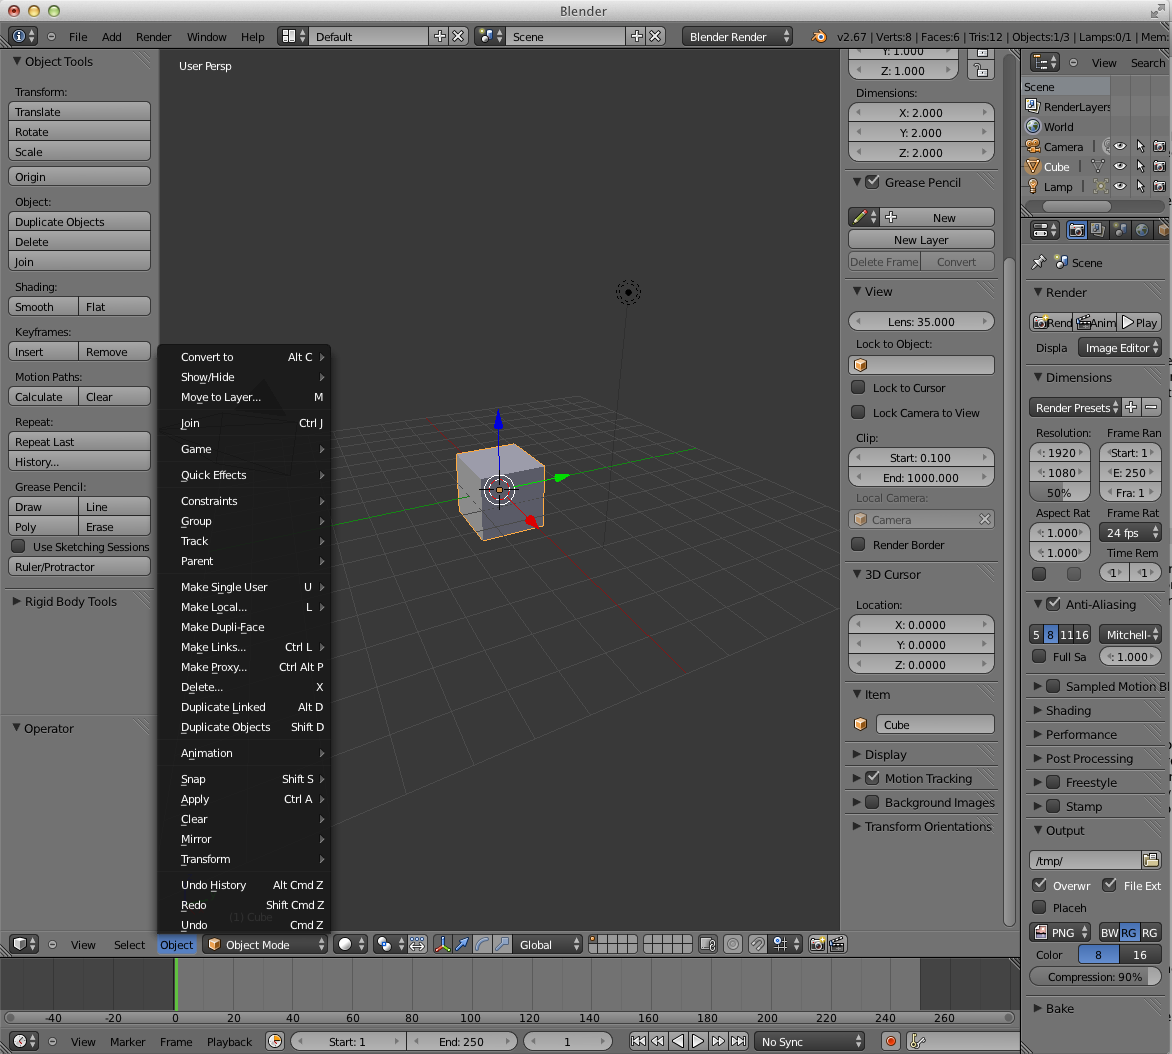
\includegraphics[width=0.9\columnwidth]{blender_interface.png}
\caption{A screenshot showing the complexity of Blender's user interface.}
\label{fig:blender_interface}
\end{figure}

\paragraph*{Animations:}
For scientists creating animations of molecules, SketchBio provides a basic interface to a much more complex system.  Blender is a production level animation and rendering tool.  It has an extremely complex user interface with dozens of hotkeys, menus and buttons (see Figure \ref{fig:blender_interface}.  Blender also has a python scripting interface that provides access to all of its functionality.  SketchBio uses this scripting interface to create its animations and render them in a high quality rendering engine, but provides a much simpler way to access that interface.  SketchBio provides simple operations, moving along the video timeline and setting keyframes on objects.  Keyframes save not only position and orientation of the objects but also other changeable aspects such as color.  These values are then interpolated between the keyframes to produce the motion in the animation.  These values are also exported to Blender with a set of global settings for effects and position of light sources to produce a full-quality rendering.

\paragraph*{Grouping:}
Grouping of molecules into larger units is also supported to make constructing larger order structures easier.  This also allows smooth animation of objects that are moving together without the small variations that even the most careful hand-placement will create.  Copy and paste is also implemented and both single objects and groups can be copied and pasted, even between sessions.

\paragraph*{Importing Molecules:}
SketchBio generates molecular surfaces using UCSF Chimera.  This subprocess is controlled via python scripting and a custom plugin was written for Chimera's python interface to export additional data from Chimera in the VTK file format.  (This plugin was contributed back to the Chimera developers and is now part of the standard source distribution.)  This data includes residue and chain identifier that map to a specific location on the surface and electrostatic potential on the surface.  SketchBio uses these data sets to color the objects to be like the vinculin tail on the right in Figure \ref{fig:actin_vinculin}.

\subsection*{Novel Capabilities}

To meet the needs of our collaborators, SketchBio supports novel operations beyond those available in the programs and libraries that it harnesses.  These include ``pose-mode physics" that enables rapid docking of one protein with others and a ``crystal by example" mode that enables rapid formation of polymer molecular chains.  Each of these is described, along with how they enable optimization of collision detection.  A third feature, spring-like connectors, is then described.

\paragraph*{Pose Mode Physics:}
An observation about the motions of objects in SketchBio is: for most of the time working with the program, the only objects that move are those directly being manipulated by the user.  The user may even find it annoying if the object they are moving pushes the object they are attempting to dock it with away every time they accidentally collide.  Therefore one simplification that can be made to collision detection is to employ what we call pose mode physics.  In pose mode physics, only the objects directly manipulated by the user are allowed to move.  Each other object is fixed in place and does not even move due to collision response forces.  This allows an easier time docking the molecules as the molecule not being held does not get pushed away.

\paragraph*{Pose Mode Physics and Collision Detection:}
In pose mode, collision tests between objects that the user is not interacting with can be skipped because these objects do not move.  The only way that those objects could be in collision was if they were already in collision before.  If the collision response failed to fix the collision then, it will not fix it now, so their tests can be skipped.  This means that only collisions involving the objects that the user is moving need to be checked.  This reduces the number of collision tests to $m*n$ where m is the number of objects that the user is currently moving.  The typical number of objects that the user moves at a time is 1 or a small constant in the case of moving a group, which reduces the number of collision tests needed to $\mathcal{O}(n)$ in this expected case.

\begin{figure}[h]
\centering
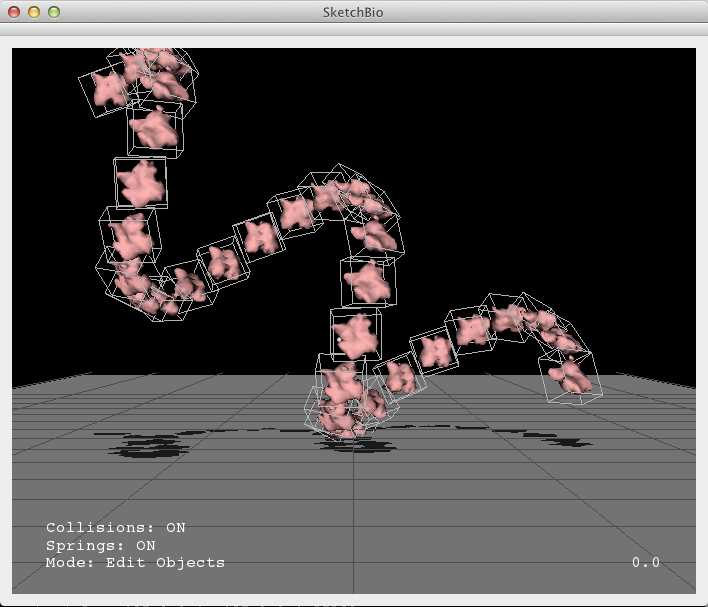
\includegraphics[width=0.9\columnwidth]{crystalByExample.png}
\caption{Crystal-by-example illustrating how a helix might be formed.}
\label{fig:crystal_by_example}
\end{figure}
\paragraph*{Crystal-by-example:}
Repeated structures that are formed from a single type of protein are common in biology (actin, microtubules, fibrin, etc.), so the ‘crystal-by-example' feature was added.  Our collaborators wanted to construct variants of such structures to study the changes caused by mutant proteins and to understand their native packing for comparison to TEM images.

This feature uses two copies of a molecule (A and B) to define an entire repeated structure.  Given $T_A$ and $T_B$, the transformation matrices that define the positions of A and B relative to the world origin, the transformation from A's coordinate system to B's coordinate system, $T_{AB} = T_A^-1*T_B$, can be computed.

B's position can be rewritten $T_B = T_A*T_{AB}$.  The next repeated molecule, C, has position $T_C = T_B*T_{AB} = T_A*T_{AB}^2$.  This can be extended to generate arbitrary numbers of molecules in a structure that is determined simply by the first two.

Many biological structures including actin fibers and microtubules form in structures that can be defined this way.  Figure \ref{fig:crystal_actin} shows an actin fiber generated this way in SketchBio.  By allowing live updates of the entire structure as the initial two objects are manipulated, SketchBio allows the scientist to explore possibilities of these structures in real time.  Some of these structures have a known transformation from one molecule to the next.  Similar to many other programs, SketchBio lets the user input the transformation to use between any two molecules to provide more accurate construction of structures with known transformations.

\begin{figure}[h]
\centering
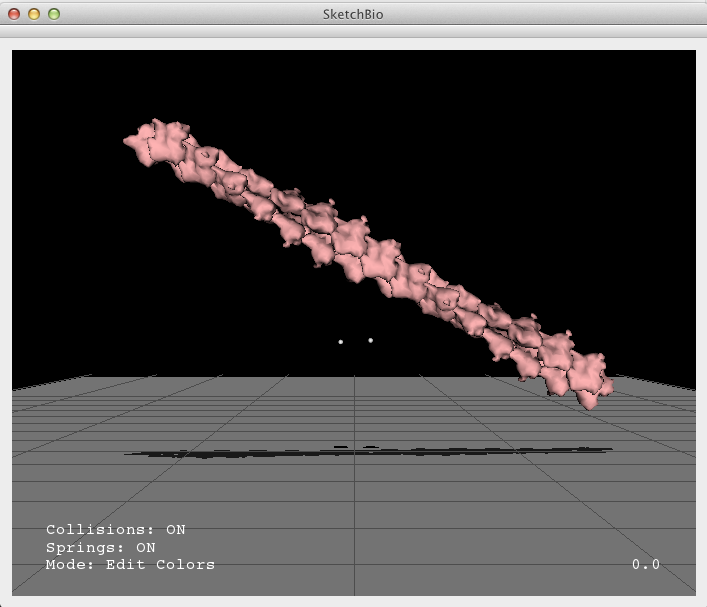
\includegraphics[width=0.9\columnwidth]{crystal_actin.png}
\caption{Actin filament created with the crystal-by-example function using the transformation matrix from the PDB data from one monomer to the next.}
\label{fig:crystal_actin}
\end{figure}

\paragraph*{Crystal-by-example Collision Detection:}
There are two ways that the user can interact with a crystal-by-example structure: moving the entire structure as a unit, or adjusting the internal transformation to change the shape of the structure.  In the first case, only collision tests between the structure and the other objects in the scene need to be done, and the above bound applies to the number of tests.  Because the structure is moved as a unit, its internal geometry does not change so if there were no internal collisions to begin with, there will be none after it was moved. 


In the second case, the internal structure does change and both internal and external collisions must be tested.  External collisions must test every object in the structure with every external object as above.

The internal case is simpler.  Let $X_i$ be the ith object in the crystal by example structure with $X_0$ and $X_1$ being the two base object in the structure.  Let $T_{i,j}$ be the transformation matrix from $X_i$ to $X_j$.  The definition of the crystal-by-example structure is that $T_{i,i+1}$ is the same for all $i$ and the geometries of all the $X_i$s are the same.  Since the geometries and transformations are the same, if there is a collision between the $ith$ and $(i+1)th$ objects anywhere in the structure, then there is also a collision between the $0th$ and $1st$ objects.  Thus testing only this one pair performs the work of n-1 tests where n is the number of objects in the structure.  This same argument holds for any $i$ and $i+k$, the $0th$ and $kth$ objects have the same relative positions and the same collisions.  Thus only the $0th$ object in the structure needs to be tested against the others which allows $\mathcal{O}(n)$ tests to suffice for all internal collisions in a repetitive structure of $n$ elements.

%\begin{figure*}[t!]
%  \centering
%  \includegraphics[height=3.5in]{placeholder.eps}
%  \caption{Example two-column figure. To insert a single column figure, remove the * in the two figure tags. }
%  \label{fig:interface}
%\end{figure*}

\paragraph*{Connectors:}
SketchBio also has connectors that can be added between objects.  These can act like springs and apply forces to keep objects positioned relative to each other or they can simply indicate that two objects are connected.  For many proteins there are regions for which the structure is unknown and these regions can be represented with these connectors.  SketchBio does not attept to simulate full molecular-dynamics forces on the molecules it displays (this would make real-time modeling impossible); instead, only a linear-spring model is applied and an extremely viscous fluid is assumed which removes momentum effects.

When acting as springs, connecters can have non-zero rest length.  When editing a set of proteins some of whose separations are known experimentally (through two-color fluorescence labeleing, FRET, or other techniques), this can be used to specify soft constraints on the 3D layout of the proteins, guiding the scientist away from impossible structures.

\subsection*{Architecture}

The architecture of SketchBio is shown in Figure \ref{fig:architecture}.  Objects can be loaded into SketchBio as .obj files from any program that writes this format or directly through the GUI (via harnessing UCSF Chimera from the PDB or a local .pdb file).  Because VTK is used in SketchBio, any file format that VTK can read can be imported with relatively minor changes.  Exporting data to Blender is done by writing a script to be run on Blender's python interface to produce the animation.  When exporting to MicroscopeSimulator, SketchBio writes out a Microscope Simulator XML project file and loads the project into MicroscopeSimulator.  SketchBio harnesses external programs when possible (PyMOL, Chimera, Blender) and uses existing libraries for other core functions (VTK, PQP, VRPN).  It maps from dozens of controls in Chimera and hundreds of controls in Blender down to 4 input options and about 20 animation controls to streamline the tasks needed for creating structures and animations.  This provides a streamlined workflow that is easy to learn and use.

\begin{figure*}[ht]
    \begin{center}
    \noindent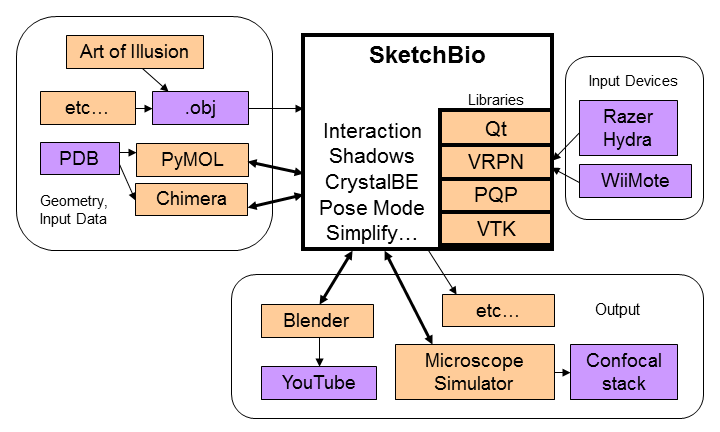
\includegraphics[width=0.9\textwidth]
    {system_diagram.png}
    \end{center}
\caption{Architecture.  SketchBio harnesses existing libraries and programs (shown in pink) to avoid replicating existing state-of-the-art algorithms.  It also makes use of standard file formats, devices, and services (shown in purple) to provide maximum interoperability with existing modeling, rendering, and analysis workflows.  Some techniques are internal, some are harnessed to appear to the user as internal (double arrows) and some are accessed via standard formats.  SketchBio currently includes three types of output: real-time rendering for model and structure comprehension, high-quality offline rendering for animation (through Blender), and simulated confocal microscopy stacks for analysis and comparison to experiment (through UNC's Microscope Simulator).  It includes custom code only for the real-time interaction, animation, and modeling portions and for its novel features.}
\label{fig:architecture}
\end{figure*}

\subsection*{Design Decisions}
We list here some design decisions that helped SketchBio achieve its goals.

\paragraph*{Harness, don't re-implement:} The design of SketchBio avoids reimplementing existing features where possible, instead using python scripting to control subprocesses to perform these operations.  When reading in PDB files, instead of writing a PDB file reader, SketchBio calls UCSF Chimera as a subprocess to read in the protein and create a displayable surface from it.  Instead of writing a new rendering library, SketchBio uses the python scripting interface of Blender to create a Blender project that will produce the desired animation.  SketchBio uses the open source Qt and VTK\cite{VTKbook} libraries for its user interface and internal rendering and the open source Proximity Query Package (PQP) for collision detection \cite{PQP}.  The VRPN library is used to communicate with the Razer Hydra input device \cite{taylor2001vrpn}.

\paragraph*{Usable in-house:} We have in the past built high-performance molecular graphics applications for scientists that used head-tracked stereo, wide-area tracking systems, and force-feedback displays.  \cite{Arthur}\cite{Grant1998}\cite{Marshburn2005}\cite{Taylor1999}\cite{Taylor1997}\cite{Taylor1993}  The scientists who were willing to travel to our laboratories to use them received great benefit, but we wanted SketchBio to be more broadly available.  Therefore, a key goal of SketchBio is to be an application that a scientist can run in their current computers.  To maximize its impact, SketchBio is designed to run on a laptop or desktop system such as a scientist would have at home or in their laboratory and uses inexpensive commercial input devices.

\paragraph*{Exploit multi-core:} SketchBio aims to minimize and consolidate the time that the scientist spends in front of the computer by running many jobs in the background.  Almost all systems in use in labs have multiple processors and in many cases the background processors can be utilized without interfering with other applications.  SketchBio takes advantage of this in two ways: using background threads to do non-immediate work and calling subprocesses to perform tasks that are already implemented externally.  This allows the scientist to avoid waiting on non-essential background output--to continue working and to perform long-running operations in the background while they work on other things.

As computers increasingly use multicore processors, SketchBio will take advantage of the background CPUs to do work that is not immediately necessary.  This can include calls to other applications in the background to precompute results or even to create images to be rendered.  This works well with the goal of utilizing other existing programs as subprocesses of SketchBio since these subprocesses can use the background CPUs without affecting SketchBio's responsiveness.

\section*{Results and Discussion}
SketchBio has been used by a several scientists and has demonstrated success in meeting its design goals.

\begin{figure}[h]
\centering
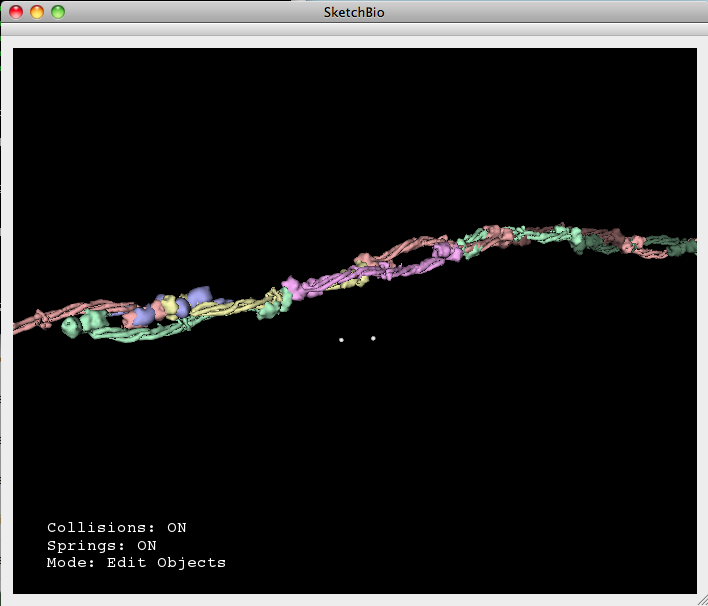
\includegraphics[width=0.9\columnwidth]{joe_test.png}
\caption{A view of the model Joe Hsiao created with SketchBio to compare usibility with UCSF Chimera}
\label{fig:joe_test}
\end{figure}

\subsection*{Use Case}
Collaborator Peter Thompson, a biochemisty graduate student, created an animation of vinculin binding to an actin fiber.  The animation is based on the model presented in a recent paper.  He was able to create the video with minimal help from a computer scientist and plans to use it in an upcoming talk.  The model in SketchBio is shown in Figure \ref{fig:peter_model} and a frame from the resulting video at approximately the same time is shown in Figure \ref{fig:peter_video}.   This animation was based on a model from a paper he had read and wished to present.

Peter also created a model based on a second paper using the charge-colored surfaces to gain a better understanding of the proposed model.

He reports that its improved quality over Powerpoint-based animations and ease of use make learning SketchBio worth the effort to a scientist that wants to make more than one animation.

\begin{figure}[h]
\centering
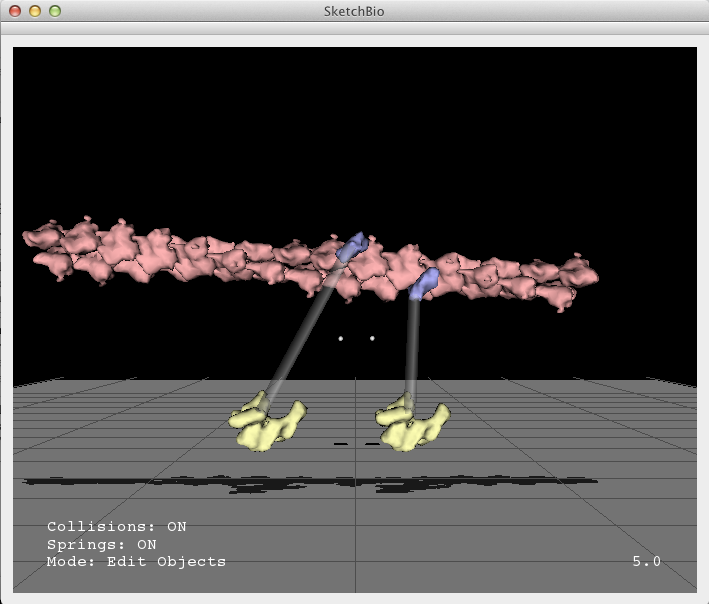
\includegraphics[width=0.9\columnwidth]{peter_model.png}
\caption{A scene from a video created by Peter Thompson in SketchBio.  Approximately the same timestep is shown rendered at its full resolution in Figure \ref{fig:peter_video}}
\label{fig:peter_model}
\end{figure}

\begin{figure}[h!]
\centering
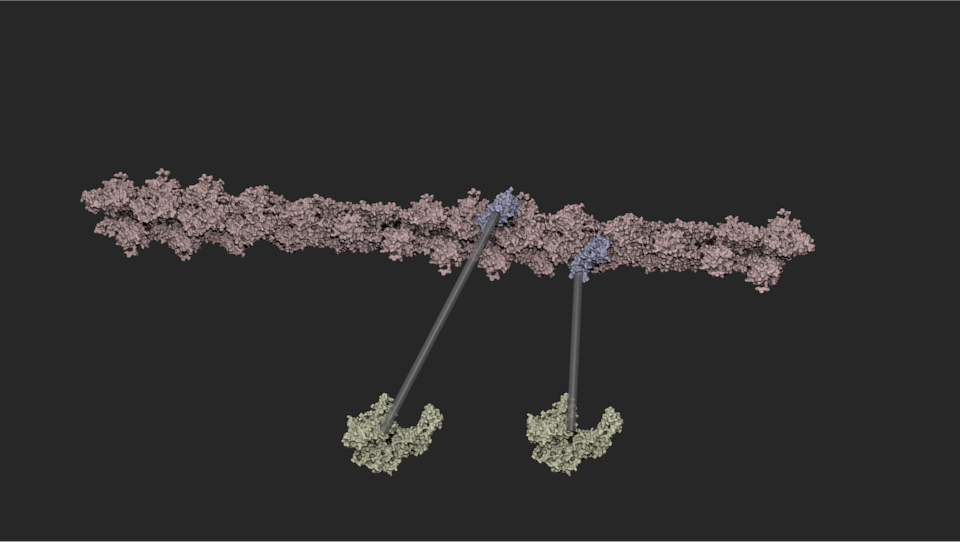
\includegraphics[width=0.9\columnwidth]{peter_video.png}
\caption{A frame from the video created by Peter Thompson.  This shows the tail domains of vinculin binding to an actin filament and slowing its motion.  This video was created in SketchBio as seen in Figure \ref{fig:peter_model} and rendered via the export to Blender feature.}
\label{fig:peter_video}
\end{figure}

\subsection*{Success Metrics}
% some wording borrowed from renewal proposal
Our primary success metric is the extent to which collaborators are able to use SketchBio themselves to construct models and animations for which they previously required programmers.  A secondary success metric is the speed at which they are able to construct these models and animations.  Our tertiary success metric is the extent to which we are able to to reuse existing functionality instead of reimplementing it within SketchBio.

To measure the ability of scientists to learn and use the system, we showed SketchBio to a visiting graduate student from NIH.  She is interested in using the system to study the proteins involved in cell focal adhesions.  After a 30-minute training session where she saw us using the system, she was able to use SketchBio to load, replicate, and placing the molecules into relevant configurations.  After similar initial training, and with access to the manual, Peter Thomson has used the system to generate both a static multi-protein model from the literature and a video showing how vinculin may separate to slow actin (see Figure \ref{fig:peter_video}).   This indicates that a series of brief training videos plus the online manual should suffice to get new users started, and that scientists are able to use SketchBio on their own.

To measure the speed of model construction, we repeated a task on SketchBio that had been done beforehand.  Constructing the protofibril models for Susan Lord took Resource computer scientist Joe Hsiao 3-3.5 hours by hand-editing transformations within Chimera (a task challenging to teach to biologists).  Using an early prototype of SketchBio, he constructed the protofibril seen in Figure \ref{fig:joe_test} in 1.5 hours (a task we'd expect a collaborator to do just as rapidly).  From this demonstration the lack of depth cues became apparent.  With the addition of the shadow plane below the objects to give better depth information and other features, Joe constructed the model in 35 minutes after about an hour of training.  In all cases, the desired model was known a-priori; all cases measure time on task and do not count the time spent learning how to use the tool.  In this case, SketchBio enabled model creation about 6 times as fast for a case of interest to our collaborators.

A direct comparison between SketchBio and an existing production pipeline for a full animation is impractical due to the amount of effort required.  To measure the effectiveness of SketchBio for the rapid construction of animations, we used it to create an animation of actin and vinculin (see supplemental materials).  We were able to load the molecules, replicate them, place them, plan camera and motion paths, and start rendering in half an hour.  The first-person design view and available pre-animation were crucial to this process, enabling design intent to be translated into action and evaluated rapidly enough to enable fluid iteration and planning.

To measure the re-use of functionality, we compare (1) the number of state-of-the-art operations harnessed from existing tools: Chimera (connecting to the protein data bank, parsing PDB file, selecting subunits, generating surfaces, generating data sets on the surfaces, simplifying surfaces), Blender (surface rendering, directional illumination, transparency, ambient occlusion, parallel rendering, frame storage), and Microscope Simulator (point-spread-function 3D blurring, TIFF stack generation); (2) the number of internally-used existing libraries: VRPN (reading from general peripheral devices), PQP (multi-object collision detection), VTK (geometric operations, real-time rendering, level-of-detail rendering, object positioning, spline interpolation); and (3) custom operations (crystal by example, pose-mode physics, drop shadows, bimanual interaction modes, spring connectors, grouping and animation).  We find that most of the operations are supported by existing tools.  Furthermore, the scripting interfaces enable rapid inclusion of additional features from external programs without re-implementation.


\section*{Limitations and future work}
Our collaborators' projects have so far involved hand-placed molecules of density sufficient small to be understood when all of them are visible.  Thus, SketchBio does not yet support automatically-placed molecules to fill the space, nor does it require complex occlusion-handling procedures.  As the user base grows, we expect to need to harness importance-based rendering techniques and autofill algorithms to handle this large number of background molecules.

SketchBio currently lacks an internal mechanism to do modeling of structures not found in the PDB.  This can be done using external modeling tools and importing models from .obj files, but collaborators have indicated that the ability to create ellipsoids whose orientation and per-axis flatness would be a way to rapidly fill in notional structures without having to leave the workflow.  We expect this to be included in the next month.

To avoid dependence on a particular hardware vendor, SketchBio is being actively ported to use a pair of Nintendo WiiMote controllers instead of the Razer Hydra controller.  Its use of the VRPN library supports switching devices by renaming the device and input for each function; a general-purpose mapping layer is being added that reads from a configuration file to enable the user to customize this remapping.  This will enable new SketchBio users to continue to use the tool until the next-generation Razer Hydra is released.

\section*{Conclusions}
SketchBio is a new tool that enables scientists to rapidly construct and validate hypothetical macromolecular structures, to animate these structures, and to produce high-quality rendered animations.  It has been tested and shown to meet its design goals:
\begin{description}
  \item[$\bullet$ Easy to learn and use.] Scientists can construct models and animations on their own.
  \item[$\bullet$ Supports iterative design.] Structures and animations can be rapidly constructed, modified, and tested.
  \item[$\bullet$ Avoids reimplementation.] State-of-the-art tools and methods are harnessed rather than reimplemented.
\end{description}

SketchBio includes state-of-the art bimanual interaction, drop shadows to improve depth perception, and other standard modeling and animation behaviors (grouping, spline interpolation, level-of-detail rendering, rapid collision detection, real-time preview).

SketchBio also includes novel interaction and computational techniques that directly support the construction of macromolecular structures: crystal by example and pose-mode physics both provide improved modeling capabilities and both enable more-rapid collision detection.  Spring connectors show unspecified interactions and support semi-automatic structure formation.

SketchBio is being released as open-source software.  It is built using portable libraries and has been compiled and used on Windows, Mac OS X and Ubuntu Linux.

\subsection*{Acknowledgements}
This work was supported by NIH grant 5-P41-EB002025.

Molecular graphics and analyses were performed with the UCSF Chimera package. Chimera is developed by the Resource for Biocomputing, Visualization, and Informatics at the University of California, San Francisco (supported by NIGMS P41-GM103311).

3D rendering was performed using Blender (blender.org). Blender is an open source project supported by the Blender Foundation and the online community.

Early versions of SketchBio used PyMOL (pymol.org) to import data from the PDB.  PyMOL is an open source project maintained and distributed by Schrödinger.

%%%%%%%%%%%%%%%%%%%%%%%%%%%%%%%%%%%%%%%%%%%%%% 
%%                                          %%
%% Backmatter begins here                   %%
%%                                          %%
%%%%%%%%%%%%%%%%%%%%%%%%%%%%%%%%%%%%%%%%%%%%%%

\begin{backmatter}

\section*{List of abbreviations used}
PQP: \textit{Proximity Query Package}, VRPN: \textit{Virtual Reality Peripheral Network}, PDB: \textit{protein data bank}.

\section*{Competing interests}
The authors declare that they have no competing interests.


%%%%%%%%%%%%%%%%%%%%%%%%%%%%%%%%%%%%%%%%%%%%%%%%%%%%%%%%%%%%%
%%                  The Bibliography                       %%
%%                                                         %%
%%  Bmc_mathpys.bst  will be used to                       %%
%%  create a .BBL file for submission.                     %%
%%  After submission of the .TEX file,                     %%
%%  you will be prompted to submit your .BBL file.         %%
%%                                                         %%
%%                                                         %%
%%  Note that the displayed Bibliography will not          %%
%%  necessarily be rendered by Latex exactly as specified  %%
%%  in the online Instructions for Authors.                %%
%%                                                         %%
%%%%%%%%%%%%%%%%%%%%%%%%%%%%%%%%%%%%%%%%%%%%%%%%%%%%%%%%%%%%%

% if your bibliography is in bibtex format, use those commands:
\bibliographystyle{bmc-mathphys} % Style BST file
\bibliography{sources}      % Bibliography file (usually '*.bib' )

% or include bibliography directly:
% \begin{thebibliography}
% \bibitem{b1}
% \end{thebibliography}

%%%%%%%%%%%%%%%%%%%%%%%%%%%%%%%%%%%
%%                               %%
%% Figures                       %%
%%                               %%
%% NB: this is for captions and  %%
%% Titles. All graphics must be  %%
%% submitted separately and NOT  %%
%% included in the Tex document  %%
%%                               %%
%%%%%%%%%%%%%%%%%%%%%%%%%%%%%%%%%%%

%%
%% Do not use \listoffigures as most will included as separate files

%\section*{Figures}
%  \begin{figure}[h!]
 % \caption{\csentence{Sample figure title.}
  %    A short description of the figure content
   %   should go here.}
   %   \end{figure}

%\begin{figure}[h!]
 % \caption{\csentence{Sample figure title.}
  %    Figure legend text.}
  %    \end{figure}

%%%%%%%%%%%%%%%%%%%%%%%%%%%%%%%%%%%
%%                               %%
%% Tables                        %%
%%                               %%
%%%%%%%%%%%%%%%%%%%%%%%%%%%%%%%%%%%

%% Use of \listoftables is discouraged.
%%
%\section*{Tables}
%\begin{table}[h!]
%\caption{Sample table title. This is where the description of the table should go.}
 %     \begin{tabular}{cccc}
%        \hline
 %          & B1  &B2   & B3\\ \hline
 %       A1 & 0.1 & 0.2 & 0.3\\
 %       A2 & ... & ..  & .\\
 %       A3 & ..  & .   & .\\ \hline
 %     \end{tabular}
%\end{table}

%%%%%%%%%%%%%%%%%%%%%%%%%%%%%%%%%%%
%%                               %%
%% Additional Files              %%
%%                               %%
%%%%%%%%%%%%%%%%%%%%%%%%%%%%%%%%%%%

%\section*{Additional Files}
%  \subsection*{Additional file 1 --- Sample additional file title}
%    Additional file descriptions text (including details of how to
%    view the file, if it is in a non-standard format or the file extension).  This might
%    refer to a multi-page table or a figure.

%  \subsection*{Additional file 2 --- Sample additional file title}
%    Additional file descriptions text.

\end{backmatter}
\end{document}
